%% ---------------------------------------------------------------------------
%% Packages, layout and macros. Content lives in chapters/, metadata in main.tex.
%% ---------------------------------------------------------------------------

%% Fonts and language
\usepackage[T1]{fontenc}
\usepackage{lmodern}
\usepackage[english]{babel}
\usepackage{microtype}

%% Layout
\usepackage[margin=2.5cm]{geometry}
\usepackage{indentfirst}
\usepackage{setspace}
\onehalfspacing
\emergencystretch=2em % avoid overfull lines with long names in monospace

%% Math
\usepackage{amsmath, amssymb, mathtools}

%% Figures and tables
\usepackage{graphicx}
\graphicspath{{figures/}} % 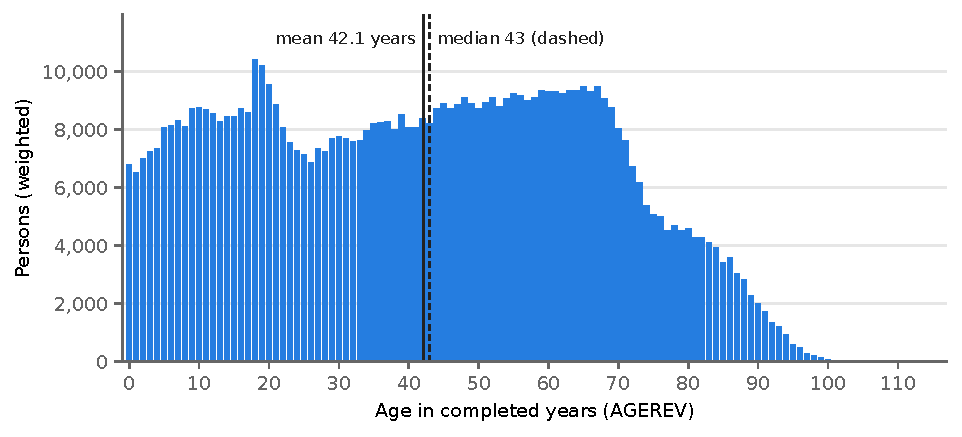
\includegraphics{age_distribution} -> figures/age_distribution.(pdf|png)
\usepackage{float}        % [H] placement
\usepackage{booktabs}
\usepackage{tabularx}
\usepackage{caption}
\usepackage{subcaption}
\usepackage{xcolor}

%% Algorithms and code listings
\usepackage{algorithm}
\usepackage{algpseudocode}
\usepackage{listings}
\lstset{
  basicstyle=\ttfamily\small,
  breaklines=true,
  frame=single,
  columns=fullflexible,
  keywordstyle=\color{blue!60!black},
  commentstyle=\color{gray},
  % listings is not UTF-8 aware: map the accented letters used in column names
  literate={é}{{\'e}}1 {è}{{\`e}}1 {à}{{\`a}}1 {ç}{{\c{c}}}1 {ô}{{\^o}}1 {É}{{\'E}}1,
}
% Python excerpts of the analysis: \begin{lstlisting}[style=py] ... \end{lstlisting}
\lstdefinestyle{py}{
  language=Python,
  basicstyle=\ttfamily\footnotesize,
  columns=fixed, basewidth=0.5em, keepspaces=true,
  stringstyle=\color{green!40!black},
  showstringspaces=false,
  aboveskip=0.6\baselineskip,
  belowskip=0.6\baselineskip,
}

%% Question / answer boxes: one per question of the assignment
\usepackage[most]{tcolorbox}
% \begin{qa}{<question as asked in the assignment>} <answer> \end{qa}
\newtcolorbox{qa}[1]{
  enhanced, breakable,
  colback=blue!3, colframe=blue!45!black, boxrule=0.6pt, arc=1mm,
  left=2mm, right=2mm, top=1mm, bottom=1mm,
  before upper={\textbf{Question.} \emph{#1}\par\smallskip\textbf{Answer.}\ },
}

%% Links -- hyperref must be loaded late, cleveref after it
\usepackage[hyphens]{url}
\Urlmuskip=0mu plus 1mu % let long data URLs stretch instead of running into the margin
\usepackage[hidelinks]{hyperref}
\usepackage[capitalise, noabbrev]{cleveref} % \cref{fig:x} -> "Figure 1"

%% ---------------------------------------------------------------------------
%% Macros
%% ---------------------------------------------------------------------------
\newcommand{\todo}[1]{\textcolor{red}{\textbf{[TODO: #1]}}} % visible placeholder
\newcommand{\code}[1]{\texttt{#1}}                          % file / identifier names

% Placeholder for a figure that a notebook will write to figures/<name>.pdf.
% Replace the call by \includegraphics[width=\textwidth]{<name>} once the file exists.
\newcommand{\figplaceholder}[2][0.9\textwidth]{%
  \fbox{\parbox[c][5cm][c]{#1}{\centering
    \todo{figure \texttt{\detokenize{#2}.pdf} not generated yet}}}}

%% Transport-demand notation (all usable in text mode as well)
\newcommand{\Oi}{\ensuremath{O_i}}                 % trips originating in zone i
\newcommand{\Dj}{\ensuremath{D_j}}                 % trips arriving in zone j
\newcommand{\Fij}{\ensuremath{F_{ij}}}             % flow from zone i to zone j
\newcommand{\dij}{\ensuremath{d_{ij}}}             % centroid distance i -> j [m]
\newcommand{\rhoij}{\ensuremath{\rho_{ij}}}        % friction term
\newcommand{\Oprime}{\ensuremath{O'_i}}            % scaled origins (Exercise 2.2)
\newcommand{\pii}{\ensuremath{p_i}}                % production weighting factor
\newcommand{\aj}{\ensuremath{a_j}}                 % attraction weighting factor
